\documentclass[a4paper, 11pt]{article}

\usepackage{enumitem}
\usepackage{graphicx}
\usepackage{hyperref}
\usepackage[utf8]{inputenc}
\usepackage{minted}

\begin{document}

\title{
	\textbf{Linked Lists in C}
}
\author{Neo Gullberg}
\date{Fall 2024}
\maketitle

\section{Introduction}
	In this assignment my task was to implement functionality for working with linked lists in C.
	One such functionality was the ability to combine lists together, by appending one linked list to the end of another.
	I needed to benchmark the time it took to append a list of varrying size to a list of fixed size,
	as well as the other way around.
	Similar to previous assignments I again had to try and find the time complexities of each benchmark.

\section{Basic Functionality of a Linked List}
	Before we can start benchmarking a linked list we of course have to implement it first.
	A linked list consists of an arbitrary number of cells, where each cell typically contains some kind of value and a reference to the next cell in the sequence.
	If the reference to the next cell is non existent, which in C is typically represented by a \texttt{NULL} pointer, it means the cell we are at is the last cell in the list.
	This is the struct I used to represent a cell in my code.
	\begin{minted}[obeytabs=true, tabsize=4]{c}
typedef struct Cell Cell;
struct Cell
{
	int item;
	Cell *next;
};
	\end{minted}
	The example code from the instructions also consisted of another struct, which represented the start of a linked list and explicitly contained a first element,
	but I chose to make due with only the one seen above since I thought it would mean less things to keep track of.

\section{Appending to a Linked List}
	\begin{minted}[obeytabs=true, tabsize=4]{c}
void Cell_append(Cell *top, Cell *bottom)
{
	if (top == NULL)
		return;
	while (top->next != NULL)
		top = top->next;
	top->next = bottom;
}
	\end{minted}
	This is the method I wrote that appends a linked list, \texttt{bottom}, to the last cell of another linked list, \texttt{top}.
	It first checks to make sure that \texttt{top} is not pointing to nothing and then traverses the list until it points at the last cell, where it then attaches \texttt{bottom}.

\section{The Benchmarks}
	\subsection{Appending to a Linked List of Fixed Size}
	First up was to benchmark appending a list of varrying size to the end of a list of an arbitrary fixed size.
	What exactly the fixed size corresponds to should not matter too much.
	However, we do not want it to be too small since then the actual time it takes might not be measureable by our clock.
	But we also do not want it to be too big since then it would take an unnecessarily long time to complete the benchmarks.
	I settled on a fixed size of 100, and that seemed to do the job.
	\begin{figure}[H]
		\centering
		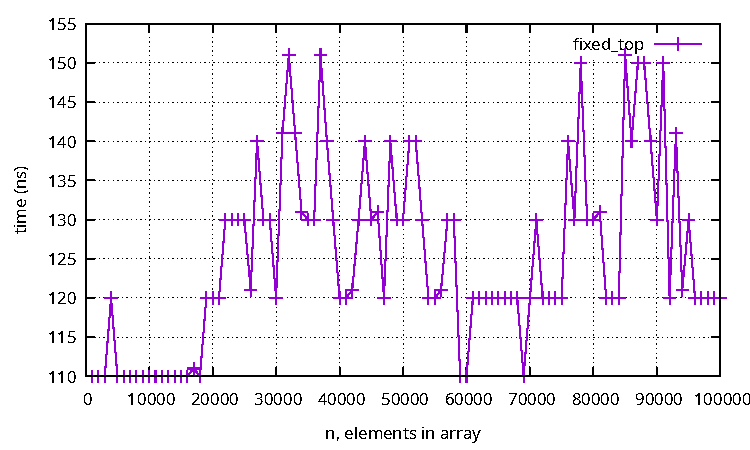
\includegraphics[scale=0.8]{graphs/fixed_top_gen_top_first.pdf}
		\caption{
			Graph showing the time it took to append a linked list of varrying size \(n\) (up to 100,000) to the bottom of a linked list of a fixed size.
			The top part generated before the bottom part.
		}
	\end{figure}
	As can be seen in \textbf{Figure 1} the time it takes to append to the bottom of a linked list seems to not grow with the size of \(n\).
	It actually seems to mimic \(O(1)\), sometimes...
	What we should be measuring is the time it takes to traverse to the last element of the fixed linked list,
	and set the next reference to be the beginning of the linked list of size \(n\).
	Should this not always take the same amount of time?
	Well the problem arises from how I created the lists.
	I started by creating the top part, and then I created the bottom part.
	This meant the cache got overflown with the bottom part.
	If we instead create the bottom part first, and then the top part, we should have the top part stored in the cache.
	\begin{figure}[H]
		\centering
		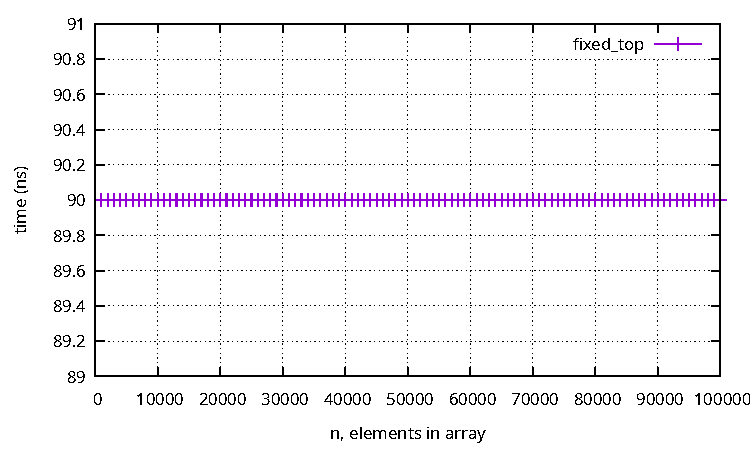
\includegraphics[scale=0.8]{graphs/fixed_top_gen_top_last.pdf}
		\caption{
			Graph showing the time it took to append a linked list of varrying size \(n\) (up to 100,000) to the bottom of a linked list of a fixed size.
			Top part generated after the bottom part.
		}
	\end{figure}
	As we can see in \textbf{Figure 2} this seemed to do to trick.
	Now it is clear that the time complexity of appending to a linked list of fixed size is \(O(1)\).

	\subsection{Appending to a Linked List of Varying Size}
	Now it is time for appending to a linked list of varying size.
	\begin{figure}[H]
		\centering
		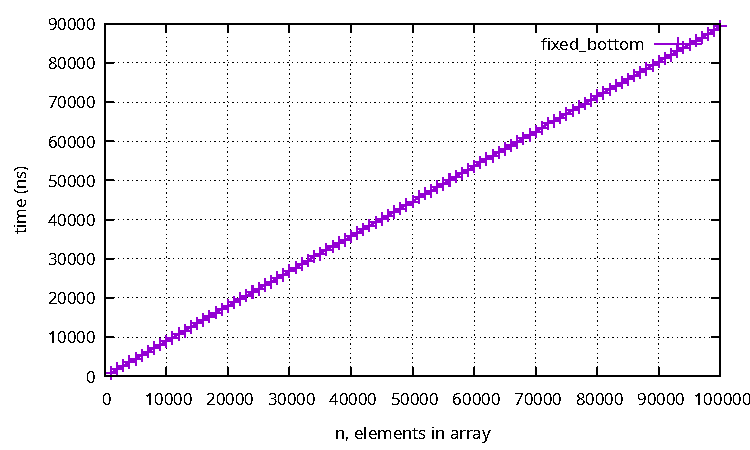
\includegraphics[scale=0.8]{graphs/fixed_bottom.pdf}
		\caption{
			Graph showing the time it took to append a linked list of fixed size to the bottom of a linked list of a varying size (up to 100,000).
		}
	\end{figure}
	The time complexity looks to be \(O(n)\), which is to be expected since we have to traverse \(n\) number of elements to get to the cell at the end where we want to append.

\section{Comparison to an Array}
	If we instead were to implement our append function for arrays it would work quite different.
	Let us say we have two arrays: one of size n, the other of size m.
	Since the elements of an array have to be located sequentially in memory, we first need to allocate memory to house n + m number of elements.
	We go through each element in the array we want at the top and add each one to the newly allocated space, then do the same for the array we want at the bottom.
	Then we would also typically want to free the space in memory that was used to store the arrays by themselves.
	It we were to append an array of size n to an array of size m, the time complexity would be \(O(n+m)\).
	The time complexity would be the same if the sizes were reversed since \(n+m = m+n\).

\section{A Stack With a Linked List}
	A stack would probably be easier to implement with a linked list instead of an array.
	The push operation would just be a renaming of the already implemented add method that I wrote for this assignment.
	The pop operation would be trivial since all we would have to do is change the first cell to be the cell that itself points to next.
	Of course we have to make sure we do not pop a \texttt(NULL) pointer, and it would probably be good practice to also free something that has just been popped.
	This time around we would not have to worry about having to neither increase nor decrease the size of an array which is nice.
	An improvement in execution time would probably come from not having to resize an array,
	but access times might be less efficient.
	But then again, in a stack we are really only interested in the top element and in that case linked lists should not be that much slower compared to an array.
	Therefore, I would guess it should improve performance to use a linked list over an array for an implementation of a stack.

\section{Source Code}
	If anyone is interested, the source code for this project can be found over at:
	\url{https://github.com/neogulgul/ID1021/tree/main/linked-list}

\end{document}
